\section{Optimum transfer}

Once direct transfers (prograde and retrograde) have been computed for each pair
of launch and arrival dates, the most optimum transfer orbit can be identified.

It is important to define the concept of optimum transfer. In this context, this
term refers to the orbit whose launch energy is the lowest. Other mission
constrains may be considered but for the purpose of this work, the launch $C_3$
energy is the only parameter considered. The reason is that the $\Delta v_1$
required for a direct transfer is a limiting factor for nowadays technology.

Porkchps represented in figures
\ref{fig:oumuamua-direct-prograde-transfer-porkchop} and
\ref{fig:borisov-direct-prograde-transfer-porkchop} contain an optimum transfer
maneuver. This section analyzes the most optimum transfer for each interloper,
including a detailed description of the trajectory and the impulses required.

\subsection{'Oumuamua}

Among the prograde and retrogade direct transfers, the most optimum transfer is
contained in the set of prograde orbits. Analyzing figure
\ref{fig:oumuamua-direct-prograde-transfer-porkchop} in detail, it is possible
to limit the value of the characteristic energy at launch to ignore high speed
impulse solutions. This reveals figure \ref{fig:oumuamua-optimum-porkchop}. The
analysis is also expanded for considering the arrival velocity. This is depicted
in figure \ref{fig:oumuamua-optimum-porkchop-avl}.

The values associated with the point with the lowest characteristic energy for
launching a spacecraft, indicated with a red cross in the figures, are collected
in table \ref{tab:oumuamua-direct-transfer-optimum}.

\begin{figure}[H]
  \centering
  \includegraphics[width=\textwidth]{static/oumuamua/direct-detailed-porkchop-tof.png}
        \caption[Detailed porkchop showing the optimum transfer for
        1I/'Oumuamua with the time of flight.]{Detailed porkchop showing the optimum transfer for
        1I/'Oumuamua. A region under 50 km$^2$/s$^2$ is found, indicating that
        a low energy transfer is possible. The porkchop is limited up to $25$
        km/s, which is a feasible value for nowadays technology.}
  \label{fig:oumuamua-optimum-porkchop}
\end{figure}

\begin{figure}[H]
  \centering
  \includegraphics[width=\textwidth]{static/oumuamua/direct-detailed-porkchop-avl.png}
        \caption[Detailed porkchop showing the optimum transfer for
        1I/'Oumuamua with the arrival velocity.]{Detailed porkchop showing the
        optimum transfer for 1I/'Oumuamua with isolines for the arrival
        velocity.}
  \label{fig:oumuamua-optimum-porkchop-avl}
\end{figure}

\begin{table}[H]
  \centering
  \begin{tabular}{|c|c|c|c|}
    \hline
    Object & Launch date & Arrival date & Required $C_3$ [km$^2$/s$^2$] \\
    \hline
    1I/'Oumuamua & 2017-01-20 & 2017-10-12 & 8.82 \\
    \hline
  \end{tabular}
  \caption{Optimum transfer orbit for a direct transfer between the Earth and 1I/'Oumuamua.}
  \label{tab:oumuamua-direct-transfer-optimum}
\end{table}

Figures \ref{fig:optimum_oumuamua_orbit_xy},
\ref{fig:optimum_oumuamua_orbit_yz}, and \ref{fig:optimum_oumuamua_orbit_xz}
represent the trajectory of the optimum transfer between Earth and 1I/'Oumuamua.
Note how the orbit lies close to the ecliptic and has a very low inclination.
This allows to take advantage of the Earth's velocity to intercept the
interloper, reducing the required energy for the transfer.

\begin{figure}[H]
  \centering
  \includegraphics[width=0.95\textwidth]{static/oumuamua/direct-optimum-transfer-xy.png}
  \caption[Top view of the direct optimum transfer orbit from Earth to 1I/'Oumuamua]{
    Top view of the direct optimum transfer orbit from Earth to 1I/'Oumuamua.
    The orbit lies close to the ecliptic, taking advantage of the Earth's
    velocity to intercept the interloper.
  }
  \label{fig:optimum_oumuamua_orbit_xy}
\end{figure}

\begin{figure}[H]
  \centering
  \includegraphics[width=0.95\textwidth]{static/oumuamua/direct-optimum-transfer-xz.png}
  \caption[Front view of the direct optimum transfer orbit from Earth to 1I/'Oumuamua]{
    Front view of the direct optimum transfer orbit from Earth to 1I/'Oumuamua.
    The inclination of the orbit is very low, maximizing the kinetic energy
    provided by the Earth.
  }
  \label{fig:optimum_oumuamua_orbit_yz}
\end{figure}

\begin{figure}[H]
  \centering
  \includegraphics[width=0.95\textwidth]{static/oumuamua/direct-optimum-transfer-yz.png}
  \caption[Side view of the direct optimum transfer orbit from Earth to 1I/'Oumuamua]{
    Side view of the direct optimum transfer orbit from Earth to 1I/'Oumuamua.
    This view shows again the low inclination of the transfer orbit.}
  \label{fig:optimum_oumuamua_orbit_xz}
\end{figure}

However, a look to figure \ref{fig:oumuamua-optimum-porkchop-avl} reveals that
the arrival velocity is very high. Even if a targeting with 'Oumuamua was
attempted, the observation time would be very short. This is also evidenced by
the impulses required for the maneuver, which are collected in table
\ref{tab:oumuamua-direct-transfer-impulses}.

\begin{table}[H]
  \centering
  \begin{tabular}{|c|c|c|c|}
    \hline
    Impulse & $\Delta v_x$ [km/s] & $\Delta v_y$ [km/s] & $\Delta v_z$ [km/s] \\
    \hline
    Launch & 0.98 & -1.16 & 2.54 \\
    \hline
    Arrival & 59.10 & -14.22 & 14.33 \\
    \hline
  \end{tabular}
  \caption{Impulses required for the optimum transfer between Earth and 1I/'Oumuamua.}
  \label{tab:oumuamua-direct-transfer-impulses}
\end{table}

The total time of flight is 265 days. The cost for the launch is around $2.96$
km/s, while the arrival impulse is $62.45$ km/s. The total cost for the transfer
is $65.41$ km/s.

\subsection{Borisov}

Regarding Borisov, the most optimum transfer is also a prograde transfer. The
analysis of figure \ref{fig:borisov-direct-prograde-transfer-porkchop} reveals a
series of periodic regions in the lower left region. The region containing the
lowest characteristic energy is shown in figure
\ref{fig:borisov-optimum-transfer-porkchop-tof}. The analysis is expanded again
to the arrival velocity, which is shown in figure
\ref{fig:borisov-optimum-transfer-porkchop-avl}.

The values associated with the point with the lowest characteristic energy for
2I/Borisov are collected in table \ref{tab:borisov-direct-transfer-optimum}.

\begin{table}[H]
  \centering
  \begin{tabular}{|c|c|c|c|}
    \hline
    Object & Launch date & Arrival date & Required $C_3$ [km$^2$/s$^2$] \\
    \hline
    2I/Borisov & 2018-07-11 & 2019-10-27 & 32.14 \\
    \hline
  \end{tabular}
  \caption{Optimum transfer orbit for a direct transfer between the Earth and 2I/Borisov.}
  \label{tab:borisov-direct-transfer-optimum}
\end{table}

\begin{figure}[H]
  \centering
  \includegraphics[width=\textwidth]{static/borisov/direct-detailed-porkchop-tof.png}
        \caption[Detailed porkchop showing the optimum transfer for
        2I/Borisov with the time of flight.]{Detailed porkchop showing the
        optmum transfer for 2I/Borisov with isolines for the time of flight. A
        region below 50 km$^2$/s$^2$ is found, similarly to the case of
        'Oumuamua.}
  \label{fig:borisov-optimum-transfer-porkchop-tof}
\end{figure}

\begin{figure}[H]
  \centering
  \includegraphics[width=\textwidth]{static/borisov/direct-detailed-porkchop-avl.png}
        \caption[Detailed porkchop showing the optimum trasnfer for 2I/Borisov
        with the arrival velocity]{Detailed porkchop showing the optimum transfer for
        2I/Borisov with isolines for the arrival velocity. Despite having found
        an optimum transfer, the arrival velocity is very high.}
  \label{fig:borisov-optimum-transfer-porkchop-avl}
\end{figure}

The total time of flight is 473 days. The total cost for the launch is around
$5.65$ km/s and the arrival impulse is $32.95$ km/s. The total cost for the
maneuver is $38.61$ km/s. All the impulses are collected in table
\ref{tab:borisov-direct-transfer-impulses}.

\begin{table}[H]
  \centering
  \begin{tabular}{|c|c|c|c|}
    \hline
    Impulse & $\Delta v_x$ [km/s] & $\Delta v_y$ [km/s] & $\Delta v_z$ [km/s] \\
    \hline
    Launch & 5.28 & 1.99 & 0.43 \\
    \hline
    Arrival & -1.71 & -18.27 & -27.37 \\
    \hline
  \end{tabular}
  \caption{Impulses required for the optimum transfer between Earth and 2I/Borisov.}
  \label{tab:borisov-direct-transfer-impulses}
\end{table}

Figures \ref{fig:optimum_borisov_orbit_xy}, \ref{fig:optimum_borisov_orbit_yz},
and \ref{fig:optimum_borisov_orbit_xz} represent the trajectory of the optimum
transfer from Earth to 2I/Borisov. Again, the transfer does not present a high
inclination, which allows the spacecraft to benefit from Earth's velocity.

\begin{figure}[H]
  \centering
  \includegraphics[width=0.95\textwidth]{static/borisov/direct-optimum-transfer-xy.png}
  \caption[Top view of the direct optimum transfer orbit from Earth to
        2I/Borisov]{
    Top view of the direct optimum transfer orbit from Earth to 2I/Borisov.
    The orbit lies close to the ecliptic, taking advantage of the Earth's
    velocity to intercept the interloper.
  }
  \label{fig:optimum_borisov_orbit_xy}
\end{figure}

\begin{figure}[H]
  \centering
  \includegraphics[width=0.95\textwidth]{static/borisov/direct-optimum-transfer-xz.png}
  \caption[Front view of the direct optimum transfer orbit from Earth to 2I/Borisov]{
    Front view of the direct optimum transfer orbit from Earth to 2I/Borisov.
    The inclination of the orbit is very low, maximizing the kinetic energy
    provided by the Earth.
  }
  \label{fig:optimum_borisov_orbit_yz}
\end{figure}

\begin{figure}[H]
  \centering
  \includegraphics[width=0.95\textwidth]{static/borisov/direct-optimum-transfer-yz.png}
  \caption[Side view of the direct optimum transfer orbit from Earth to 2I/Borisov]{
    Side view of the direct optimum transfer orbit from Earth to 2I/Borisov.
    This view shows again the low inclination of the transfer orbit.}
  \label{fig:optimum_borisov_orbit_xz}
\end{figure}


